\documentclass[12pt]{article}
\usepackage{amsmath}
\usepackage{graphicx}
\usepackage{hyperref}
\usepackage{listings}
\usepackage{color}
\usepackage{pythonhighlight}

\title{Operating System Course Report - First Half of the Semester}
\author{A class}
\date{\today}

\begin{document}

\maketitle
\newpage

\tableofcontents
\newpage

\section{Introduction}
This report summarizes the topics covered during the first half of the Operating System course. It includes theoretical concepts, practical implementations, and assignments. The course focuses on the fundamentals of operating systems, including system architecture, process management, CPU scheduling, and deadlock handling.

\section{Course Overview}
\subsection{Objectives}
The main objectives of this course are:
\begin{itemize}
    \item To understand the basic components and architecture of a computer system.
    \item To learn process management, scheduling, and inter-process communication.
    \item To explore file systems, input/output management, and virtualization.
    \item To study the prevention and handling of deadlocks in operating systems.
\end{itemize}

\subsection{Course Structure}
The course is divided into two halves. This report focuses on the first half, which covers:
\begin{itemize}
    \item Basic Concepts and Components of Computer Systems
    \item System Performance and Metrics
    \item System Architecture of Computer Systems
    \item Process Description and Control
    \item Scheduling Algorithms
    \item Process Creation and Termination
    \item Introduction to Threads
    \item File Systems
    \item Input and Output Management
    \item Deadlock Introduction and Prevention
    \item User Interface Management
    \item Virtualization in Operating Systems
\end{itemize}

\section{Topics Covered}

\subsection{Basic Concepts and Components of Computer Systems}
This section explains the fundamental components that make up a computer system, including the CPU, memory, storage, and input/output devices.

\subsection{System Performance and Metrics}
This section introduces various system performance metrics used to measure the efficiency of a computer system, including throughput, response time, and utilization.

\subsection{System Architecture of Computer Systems}
Describes the architecture of modern computer systems, focusing on the interaction between hardware and the operating system.

\subsection{Process Description and Control}
Processes are a central concept in operating systems. This section covers:
\begin{itemize}
    \item Process states and state transitions
    \item Process control block (PCB)
    \item Context switching
\end{itemize}

\subsection{Scheduling Algorithms}
This section covers:
\begin{itemize}
    \item First-Come, First-Served (FCFS)
    \item Shortest Job Next (SJN)
    \item Round Robin (RR)
\end{itemize}
It explains how these algorithms are used to allocate CPU time to processes.

\subsection{Process Creation and Termination}
Details how processes are created and terminated by the operating system, including:
\begin{itemize}
    \item Process spawning
    \item Process termination conditions
\end{itemize}

\subsection{Introduction to Threads}
This section introduces the concept of threads and their relation to processes, covering:
\begin{itemize}
    \item Single-threaded vs. multi-threaded processes
    % \item Benefits of multithreading
\end{itemize}
\subsection{File Systems}
File systems provide a way for the operating system to store, retrieve, and manage data. This section explains:
\subsubsection{Konsep File System}
\subsubsection{Atribut File}
\subsubsection{Operasi pada File}
\subsubsection{Tipe File}
\subsubsection{Struktur File}
\subsubsection{Metode Akses File}
\\File menyimpan informasi. Jika ingin file digunakan, informasi tersebut harus diakses dan dibaca ke memori. Terdapat beberapa cara mengakses informasi pada file yaitu akses berurutan (\textit{sequential access}), akses langsung (\textit{Direct access} atau \textit{relative access}) dan metode akses lain.
\begin{itemize}
    \item Akses Berurutan (\textit{Sequential Access})
        \\Akses berurutan merupakan metode akses paling sederhana. Informasi pada file diproses secara berurutan, satu \textit{record} diakses setelah \textit{record} yang lain. Metode akses ini berdasarkan model tape dari suatu file yang bekerja dengan perangkat \textit{sequential access} atau \textit{random-access}.
        \begin{figure}[h]
			\centering
			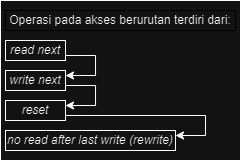
\includegraphics[width=0.5\textwidth]{asset/gambar1.png}
            \caption{Operasi akses file berurutan}
        \end{figure}
        \\Operasi read membaca bagian selanjutnya dari file dan otomatis menambah file \textit{pointer} yang melacak lokasi I/O. Operasi \textit{write} menambah ke akhir file dan ke akhir material pembacaan baru (\textit{new end of file}). File dapat di-reset ke awal dan sebuah program untuk meloncat maju atau mundur ke n \textit{record}.
        \begin{figure}[h]
			\centering
			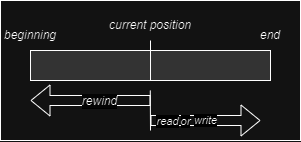
\includegraphics[width=0.6\textwidth]{asset/gambar2.png}
            \caption{Akses file berurutan}
        \end{figure}
    \item Akses Langsung (\textit{Direct Access})
        \\File merupakan \textit{logical record} dengan panjang tetap yang memungkinkan program membaca dan menulis \textit{record} dengan cepat tanpa urutan tertentu. Metode akses langsung berdasarkan model disk dari suatu file, memungkinkan acak ke sembarang blok file, memungkinkan blok acak tersebut dibaca atau ditulis.
        \begin{figure}[h]
			\centering
			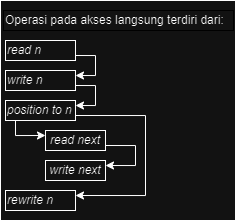
\includegraphics[width=0.6\textwidth]{asset/gambar3.png}
            \caption{Operasi akses file langsung}
        \end{figure}
        \\Operasi file dimodifikasi untuk memasukkan nomor blok sebagai parameter. Nomor blok ditentukan \textit{user} yang merupakan nomor blok relatif, misalnya indeks relatif ke awal dari file. Blok relatif pertama dari file adalah 0, meskipun alamat disk absolut aktual dari blok misalnya 17403 untuk blok pertama. Metode ini mengijinkan sistem operasi menentukan dimana file ditempatkan dan mencegah user mengakses posisi dari sistem file yang bukan bagian dari file tersebut. 
        \\Tidak semua sistem operasi menggunakan baik akses berurutan atau akses langsung untuk file. Beberapa sistem hanya menggunakan akses berurutan, beberapa sistem lain menggunakan akses langsung. Untuk mengubah akses berurutan ke akses langsung bukan sesuatu hal yang sulit seperti pada gambar di bawah.
        \begin{figure}[h]
			\centering
			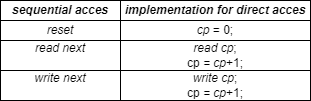
\includegraphics[width=0.6\textwidth]{asset/gambar4.png}
            \caption{Mengubah akses berurutan menjadi akses langsung}
        \end{figure}
    \item  Metode Akses Lain
        \\Metode akses lain dapat dibangun berpedoman pada metode \textit{direct access}. Metode tambahan ini biasanya melibatkan konstruksi indeks untuk file. Indeks, seperti indeks pada bagian akhir buku, berisi \textit{pointer} ke blok-blok tertentu. Untuk menentukan masukan dalam file, pertama dicari indeks, dan kemudian menggunakan \textit{pointer} untuk mengakses file secara langsung dan menemukan masukan yang tepat.
        \\File indeks dapat disimpan di memori. Bila file besar, file indeks juga menjadi terlalu besar untuk disimpan di memori. Salah satu pemecahan nya adalah membuat indeks untuk file indeks. File indeks primer berisi \textit{pointer} ke file indeks sekunder, yang menunjuk ke data item aktual. Bentuk pengaksesan secara berindeks diilustrasikan pada gambar di bawah.
        \begin{figure}[h]
			\centering
			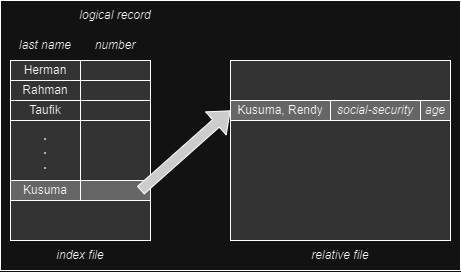
\includegraphics[width=0.7\textwidth]{asset/gambar5.png}
            \caption{Mengubah akses berurutan menjadi akses langsung}
        \end{figure}
    \end{itemize}
    \subsubsection{Struktur Direktori}
    \subsubsection{\textit{File System Mounting}}
    \\Suatu sistem file harus di-\textit{mount} sebelum diakses. File yang tidak di-\textit{mount} seperti \textit{Fiture} 6 akan dilakukan proses \textit{mounting} pada \textit{mount point} \textit{Fiture} 7.
        \begin{figure}[h!]
			\centering
			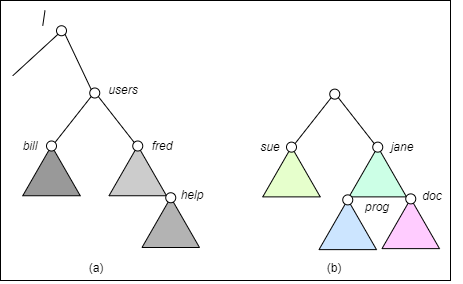
\includegraphics[width=0.6\textwidth]{asset/gambar6.png}
            \caption{(a) Sistem eksis (b) partisi yang tidak di-\textit{mount}}
        \end{figure}
        \begin{figure}[h!]
			\centering
			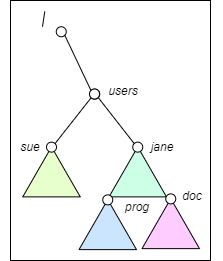
\includegraphics[width=0.6\textwidth]{asset/gambar7.png}
            \caption{\textit{Mount point}}
        \end{figure}
    \subsubsection{File Sharing}
    \subsubsection{Proteksi}
    \begin{thebibliography}{99}
        \bibitem{arpaci2018} 
        Silberschatz, Galvin \& Gagne. (2013). \textit{Operating System Concepts – 9th Edition}. cc.ee.ntu.edu.tw.
        \bibitem{Geeks} 
        GeeksforGeeks. (2024, Juny 24). \textit{File Systems in Operating System}. Retrieved from GeeksforGeeks: \textit{https://www.geeksforgeeks.org/file-systems-in-operating-system/}
    \end{thebibliography}

\subsection{Input and Output Management}
Input and output management is key for handling the interaction between the system and external devices. This section includes:
\begin{itemize}
    \item Device drivers
    \item I/O scheduling
\end{itemize}

\subsection{Deadlock Introduction and Prevention}
Explores the concept of deadlocks and methods for preventing them:
\begin{itemize}
    \item Deadlock conditions
    \item Deadlock prevention techniques
\end{itemize}

\subsection{User Interface Management}
This section discusses the role of the operating system in managing the user interface. Topics covered include:
\begin{itemize}
    \item Graphical User Interface (GUI)
    \item Command-Line Interface (CLI)
    \item Interaction between the user and the operating system
\end{itemize}

\subsection{Virtualization in Operating Systems}
Virtualization allows multiple operating systems to run concurrently on a single physical machine. This section explores:
\begin{itemize}
    \item Concept of virtualization
    \item Hypervisors and their types
    \item Benefits of virtualization in modern computing
\end{itemize}

\section{Assignments and Practical Work}
\subsection{Assignment 1: Process Scheduling}
Students were tasked with implementing various process scheduling algorithms (e.g., FCFS, SJN, and RR) and comparing their performance under different conditions.
\subsubsection{Group 1}
\begin{python}
    class Process:
    def __init__(self, pid, arrival_time, burst_time):
        self.pid = pid
        self.arrival_time = arrival_time
        self.burst_time = burst_time
        self.completion_time = 0
        self.turnaround_time = 0
        self.waiting_time = 0
\end{python}

\begin{table}[htbp] % Optional: For floating position
    \centering
    \begin{tabular}{|c|c|c|} % Defines number of columns and alignment (c = center, l = left, r = right). '|' creates vertical lines.
    \hline
    Header 1 & Header 2 & Header 3 \\ % Column headers
    \hline
    Row 1, Column 1 & Row 1, Column 2 & Row 1, Column 3 \\ % First row of data
    \hline
    Row 2, Column 1 & Row 2, Column 2 & Row 2, Column 3 \\ % Second row of data
    \hline
    \end{tabular}
    \caption{Your table caption} % Optional: For adding a caption
    \label{tab:your_label} % Optional: For cross-referencing the table
\end{table}
\subsection{Assignment 2: Deadlock Handling}
In this assignment, students were asked to simulate different deadlock scenarios and explore various prevention methods.

\subsection{Assignment 3: Multithreading and Amdahl's Law}
This assignment involved designing a multithreading scenario to solve a computationally intensive problem. Students then applied **Amdahl's Law** to calculate the theoretical speedup of the program as the number of threads increased.
\subsubsection{Group 8}
\textbf{Soal:}
\par Sebuah perusahaan teknologi sedang mengembangkan sebuah aplikasi pengolahan gambar yang memanfaatkan kemampuan komputasi \textit{multithreading} untuk mempercepat proses \textit{rendering} gambar. Aplikasi ini didesain agar bisa memanfaatkan beberapa \textit{core} CPU secara bersamaan. Salah satu developer aplikasi ini, Sarah, mendapati bahwa tidak semua bagian dari proses rendering bisa dijalankan secara paralel, karena ada beberapa bagian yang harus dijalankan secara berurutan (\textit{sequential}).
\par Sarah mendengar tentang Amdahl’s Law, yang menyatakan bahwa potensi percepatan komputasi paralel bergantung pada proporsi kode yang dapat diparalelisasi. Setelah melakukan \textit{profiling} terhadap aplikasinya, Sarah menemukan bahwa 70% dari proses \textit{rendering} dapat dijalankan secara paralel, sementara 30% lainnya harus tetap berjalan secara \textit{sequential}.
\par Perusahaan ini menggunakan mesin dengan CPU \textit{multi-core} yang memiliki 8 \textit{core} fisik, dan Sarah ingin mengetahui seberapa besar kecepatan yang bisa diperoleh dengan menggunakan 8 \textit{core} untuk bagian yang bisa diparalelisasi.
\begin{enumerate}
    \item Berapa maksimal percepatan (\textit{speedup}) teoritis yang bisa didapat Sarah jika ia menggunakan 8 \textit{core}, berdasarkan Amdahl’s Law?
    \item Jika perusahaan ingin meningkatkan proporsi paralel dari 70% menjadi 90%, berapa percepatan teoritis yang bisa didapat dengan tetap menggunakan 8 \textit{core}?
    \item Diskusikan secara umum, bagaimana Amdahl’s Law mempengaruhi strategi pengembangan perangkat lunak yang memanfaatkan \textit{multithreading}, khususnya dalam konteks aplikasi Sarah. Apakah ada batasan yang perlu diperhatikan meskipun jumlah \textit{core} CPU terus bertambah?
\end{enumerate}
\par \textbf{Jawaban:}
\par \textbf{\textit{Output}:}
\par \textbf{Kesimpulan:}

\subsection{Assignment 4: Simple Command-Line Interface (CLI) for User Interface Management}
Students were tasked with creating a simple **CLI** for user interface management. The CLI should support basic commands such as file manipulation (creating, listing, and deleting files), process management, and system status reporting.

\subsection{Assignment 5: File System Access}
In this assignment, students implemented file system access routines, including:
\begin{itemize}
    \item File creation and deletion
    \item Reading from and writing to files
    \item Navigating directories and managing file permissions
\end{itemize}

\section{Conclusion}
The first half of the course introduced core operating system concepts, including process management, scheduling, multithreading, and file system access. These topics provided a foundation for more advanced topics to be covered in the second half of the course.

\end{document}